\section{Setup and Experimental Apparatus }
\label{sec:setup}

We performed measurements of SiPM properties in the laboratory at Caltech using
signals from a class 3R PiLas laser which produces light at a wavelength of
$407$~nm. Beam measurements were performed at the H4 beam-line of the CERN
North-Area test-beam facility, which provides secondary beams of energies
ranging between $20$~GeV and $400$~GeV. The beams are composed of a mixture of
electrons and pions. The electron fraction in the beam is typically around 75\%.

The data acquisition (DAQ) system is based on a CAEN V1742 switched capacitor
digitizer~\cite{DRS4}, whose electronic time resolution has been measured to be
$4$~ps. Data readout for the laser-based measurements are triggered by an
external digital trigger signal, while at the H4 beamline readout is triggered
by a signal in a photomultiplier tube coupled to a
$3$~$\mathrm{cm}$~$\times$~$3$~$\mathrm{cm}$ plastic scintillator. A
micro-channel plate photo-multiplier (MCP-PMT) detector is used to provide a
very precise reference time-stamp in order to measure the time resolution of the 
SiPM signals.

\subsection{Setup for Laser-based SiPM Timing Measurements}

SiPMs are mounted on a printed circuit board (PCB) with a clipping capacitance
circuit shown in Figure~\ref{fig:Circuit}. The is mechanically attached to an
optical breadboard enclosed within a box lined with copper foil for RF
shielding. The laser is injected via a light-guide fiber mounted on an optical
holder. The laser beam is immediately split by a refractive mirror and half of
the light is directed straight into the MCP-PMT while the other half of the
light is directed onto the SiPM under test. A photograph of the setup is shown
in Figure~\ref{fig:laserSetup}. The Photek-240 MCP-PMT is used as the reference
time detector whose time resolution has been measured to be below $7$~ps for
beam particles~\cite{MCPShowerMaxPaper}. To cover a large range of laser beam
intensity, neutral density (ND) filters with ND number between 0.2 and 2.4
are placed between the mirror and the SiPMs under test.

\begin{figure}[htbp]
\centering
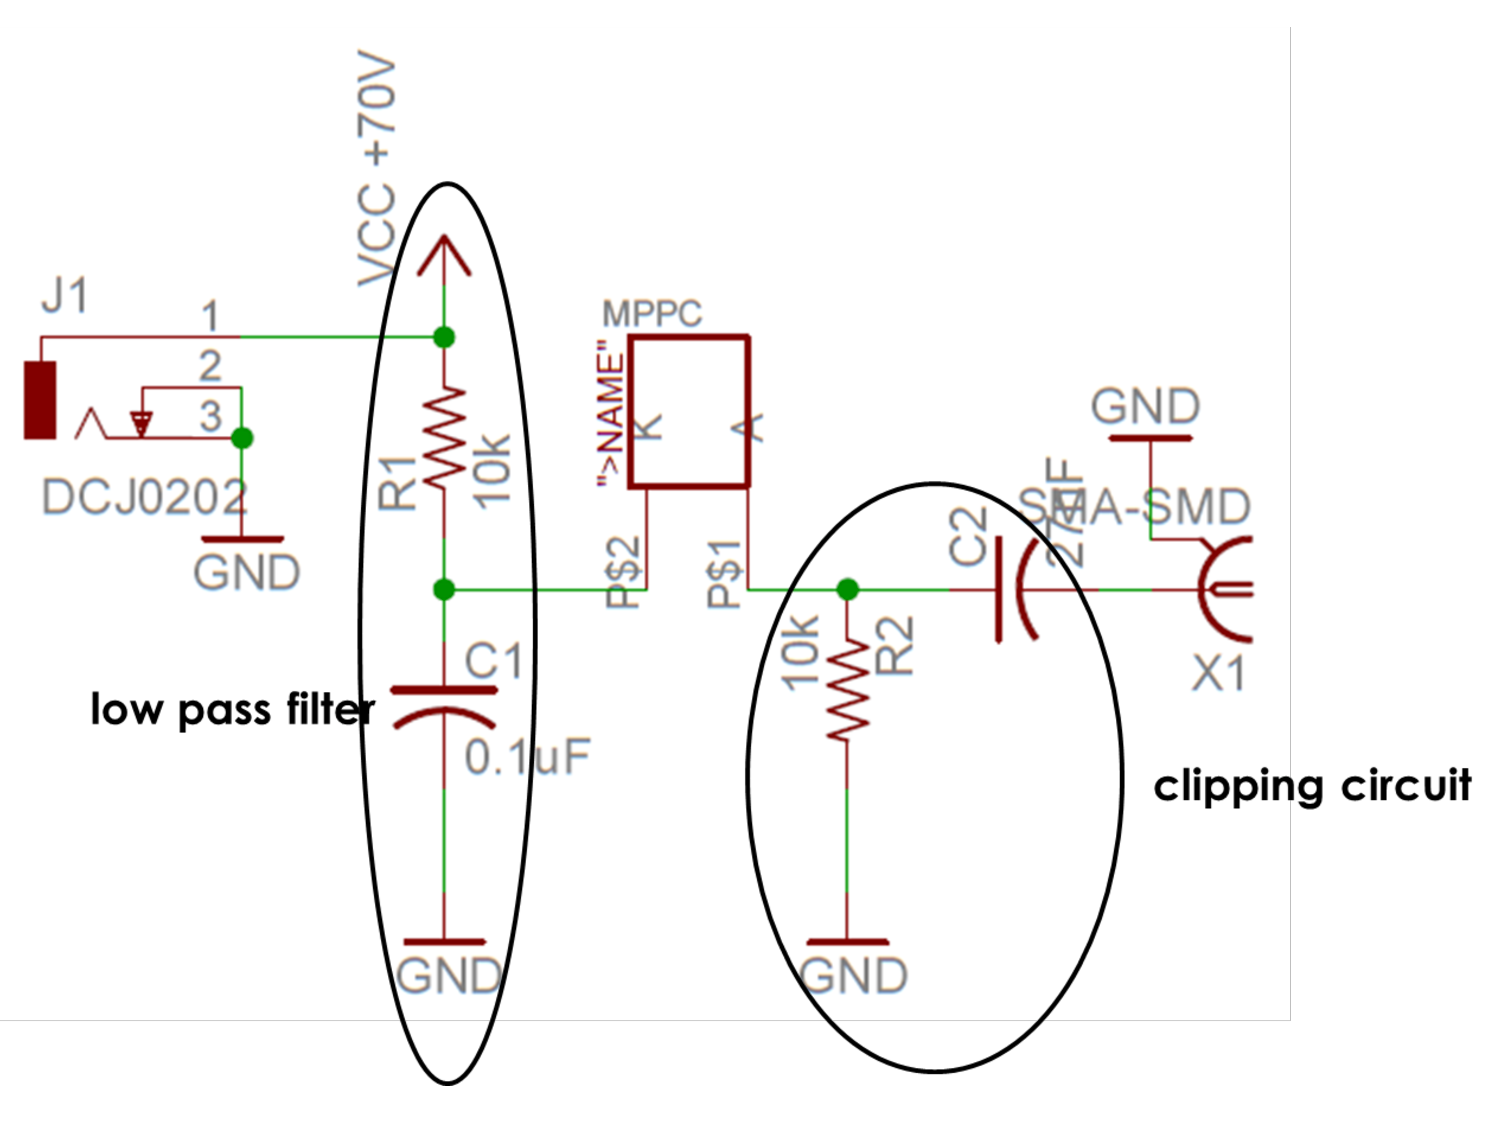
\includegraphics[width=0.49\textwidth]{figures/CircuitDiagram.pdf}
\caption{A schematic diagram of the circuit used to read out the SiPMs.}
\label{fig:Circuit}
\end{figure}


%Figure: Diagram of detector elements
\begin{figure}[htbp] 
\centering
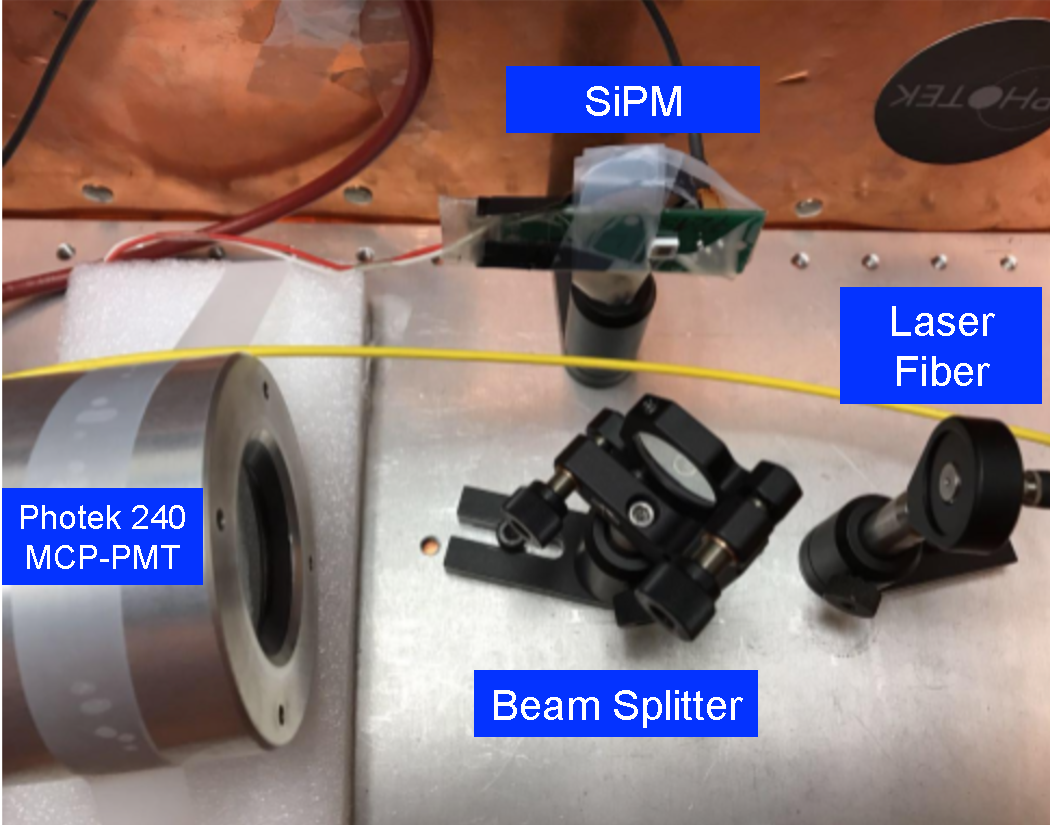
\includegraphics[width=0.49\textwidth]{figures/SiPMSetup1.pdf} 
\caption{Photograph of the Laser-based SiPM timing measurement setup.} 
\label{fig:laserSetup} 
\end{figure} 

\subsection{Setup for Timing Measurements of Scintilators with SiPM readout.}

The experimental setup we use for the calorimetric timing measurements consists
of a single cell of a sampling calorimeter with 29 alternating layers of LYSO
crystal and tungsten absorber. This arrangement is known as a Shashlik sampling
calorimeter configuration. The lateral dimensions are
$14\times14$~$\mathrm{mm}^{2}$. The total depth of the cell is about $11.5$~cm
with the LYSO plates having a thickness of $1.5$~mm. The same cell has been used
to measure the timing performance in comparison to the timing performance of a
single cube of LYSO~\cite{Anderson:2015gha}. The scintillation light from the LYSO
plates is extracted with four wave length shifting (WLS) fibers. The fibers are
coupled to four different types of Hamamatsu SiPMs with 10, 15 and 25~$\mu$m pixel size
and $1\times 1$~$\mathrm{mm}^{2}$ and $3\times 3$~$\mathrm{mm}^{2}$ sensor
size~\cite{hamamatsuMPPC}. The SiPMs are all read out with a DRS digitizer through the
clipping circuit shown above in Figure~\ref{fig:Circuit}. The same clipping circuit is 
used for all four SiPMs. We do not amplify the output
signal of the SiPMs, only exploiting the very large light yield of the LYSO
scintillator and the intrinsic amplification of the SiPMs. A labeled photograph
of the setup in the H4 beamline is shown in Figure~\ref{fig:TestbeamSetup}
below. More details of the calorimetric performance of the Shashlik
configuration are discussed in references~\cite{shashlik1}~and~\cite{shashlik2}.

%Figure: Diagram of detector elements
\begin{figure}[htbp] 
\centering
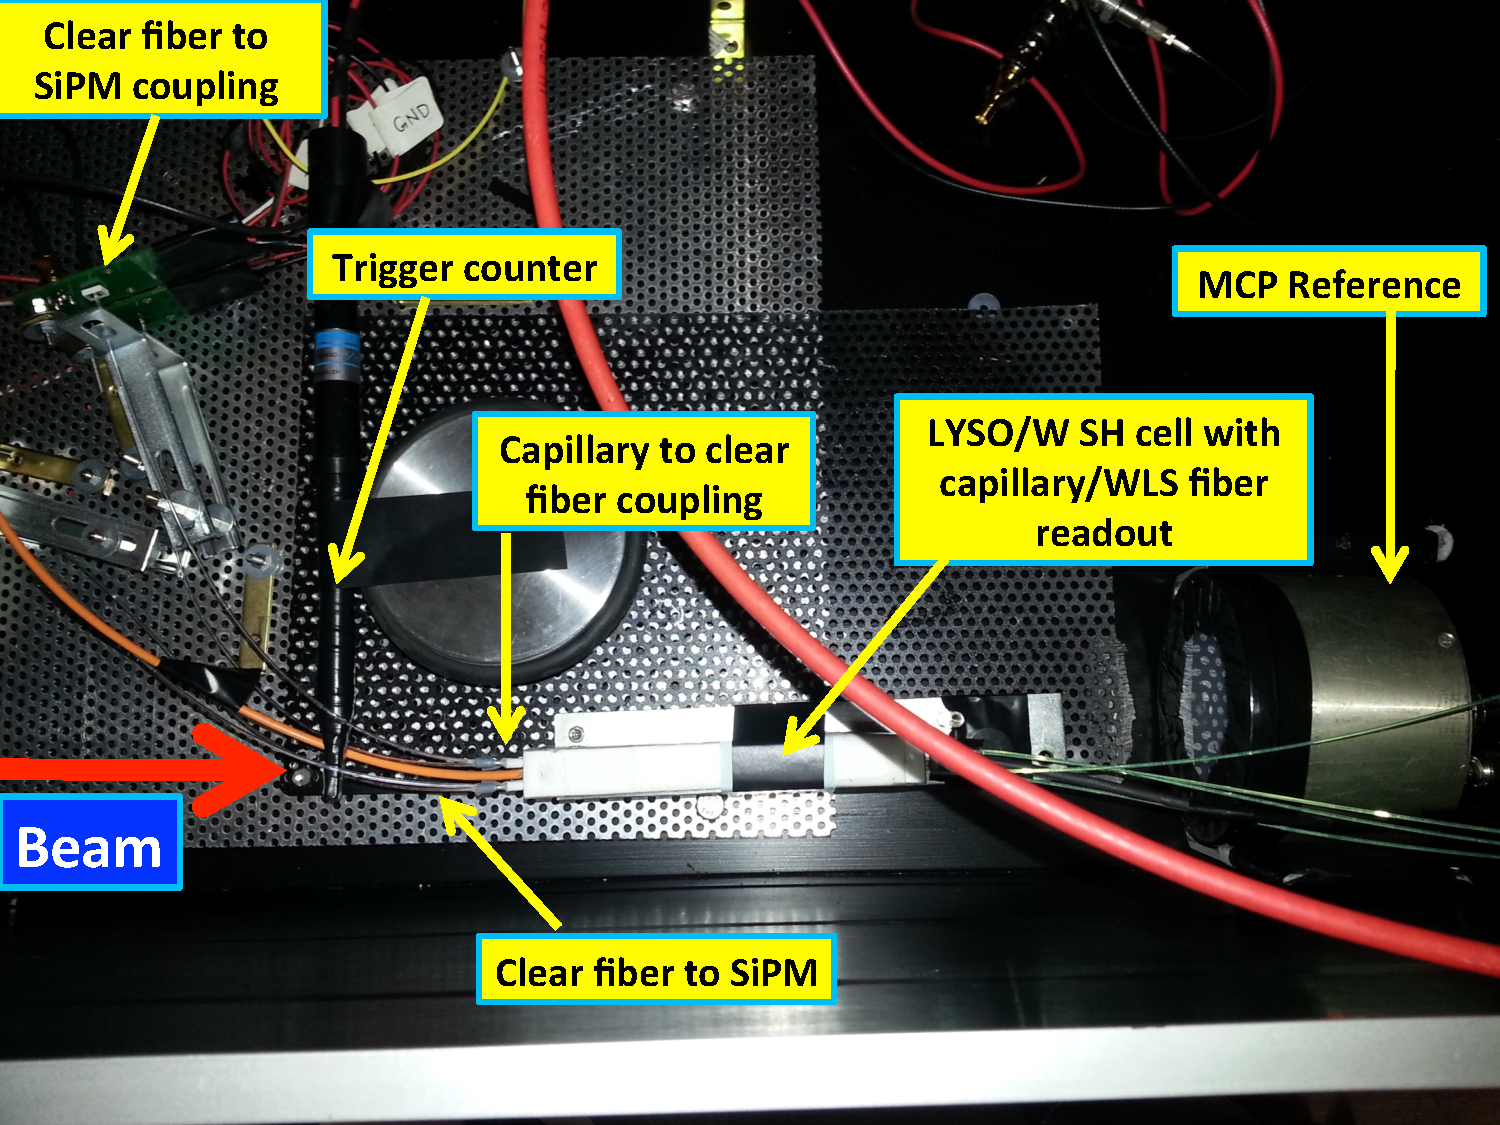
\includegraphics[width=0.95\textwidth]{figures/ShashlikTBSetupDiagram} 
\caption{Photograph of the timing measurement setup in the H4 beamline.} 
\label{fig:TestbeamSetup} 
\end{figure} 

In addition to plastic WLS fibers we also tested quartz capillaries filled with
liquid wave length shifter using DSB as a wave length shifting
agent~\cite{Baumbaugh:2016vcg}. To optically couple the quartz capillaries to the
SiPMs we use a clear plastic fiber light guide which is connected to the end of
the quartz capillary with a metal sleeve tube. The same clear fiber coupler is
used for the plastic WLS fibers to maintain equivalent light collection
efficiency. The ratio of the light collection efficiency between the plastic
fibers and the quartz capillaries approximately scales with the ratio of the
diameter of the plastic fiber and the liquid core of the quartz capillary. This
ratio is about $3$ for the fibers and capillaries we used.

As a timing reference we use a Photek 240 MCP-PMT. It is placed behind the
calorimeter cell and detects secondary shower particles escaping from the
Shashlik calorimeter cell as we did in our previous studies \cite{Anderson:2015gha}.
The time resolution is extracted by measuring the time difference between the
reference counter and the calorimeter cell over an ensemble of shower events.
The time stamp for the reference counter and calorimeter cell is extracted
from a Gaussian fit to the peak and a linear fit to the rising edge, 
respectively, as described below in Section~\ref{sec:reco}.

We measure the timing performance of the calorimeter cell with high energy
electrons in a range between $20$~GeV~and~$200$~GeV in the CERN North Area test
beam. The impact point of the electrons onto the calorimeter cell is measured
with a fiber hodoscope with a precision of better than $1$~mm. As timing measurements are
affected by shower containment, we restrict the time measurements to events
whereT shower containment is large by extracting time measurements only from 
events where the beam particle impacts in the center of the calorimeter
cell within a restricted area between $2\times2$~$\mathrm{mm}^{2}$ 
and $6\times8$~$\mathrm{mm}^{2}$ depending on the exact setup. 

\subsection{Timestamp Reconstruction}
\label{sec:reco}
The time-stamp for all signals is reconstructed by fitting the pulse waveform
with an appropriate functional form. For signal pulses from the MCP-PMTs, which
exhibit a very fast rise and decay, we fit a Gaussian function to a $1.4$~ns
window around the peak of the pulse and extract the time-stamp as the mean
parameter of the Gaussian function. For signal pulses from the SiPM sensors, we
fit a linear function to time sample points between $10\%$ and $60\%$ of the
pulse maximum and the time-stamp is assigned as the time at which the fitted
linear function rises to $20\%$ of the pulse maximum. More details of the
time-stamp reconstruction can be found in reference~\cite{Anderson:2015gha}.
